\chapter{Architecture of Fog VDN}
\label{chap:chap-three}
\begin{figure}[htbp]
\centering
	  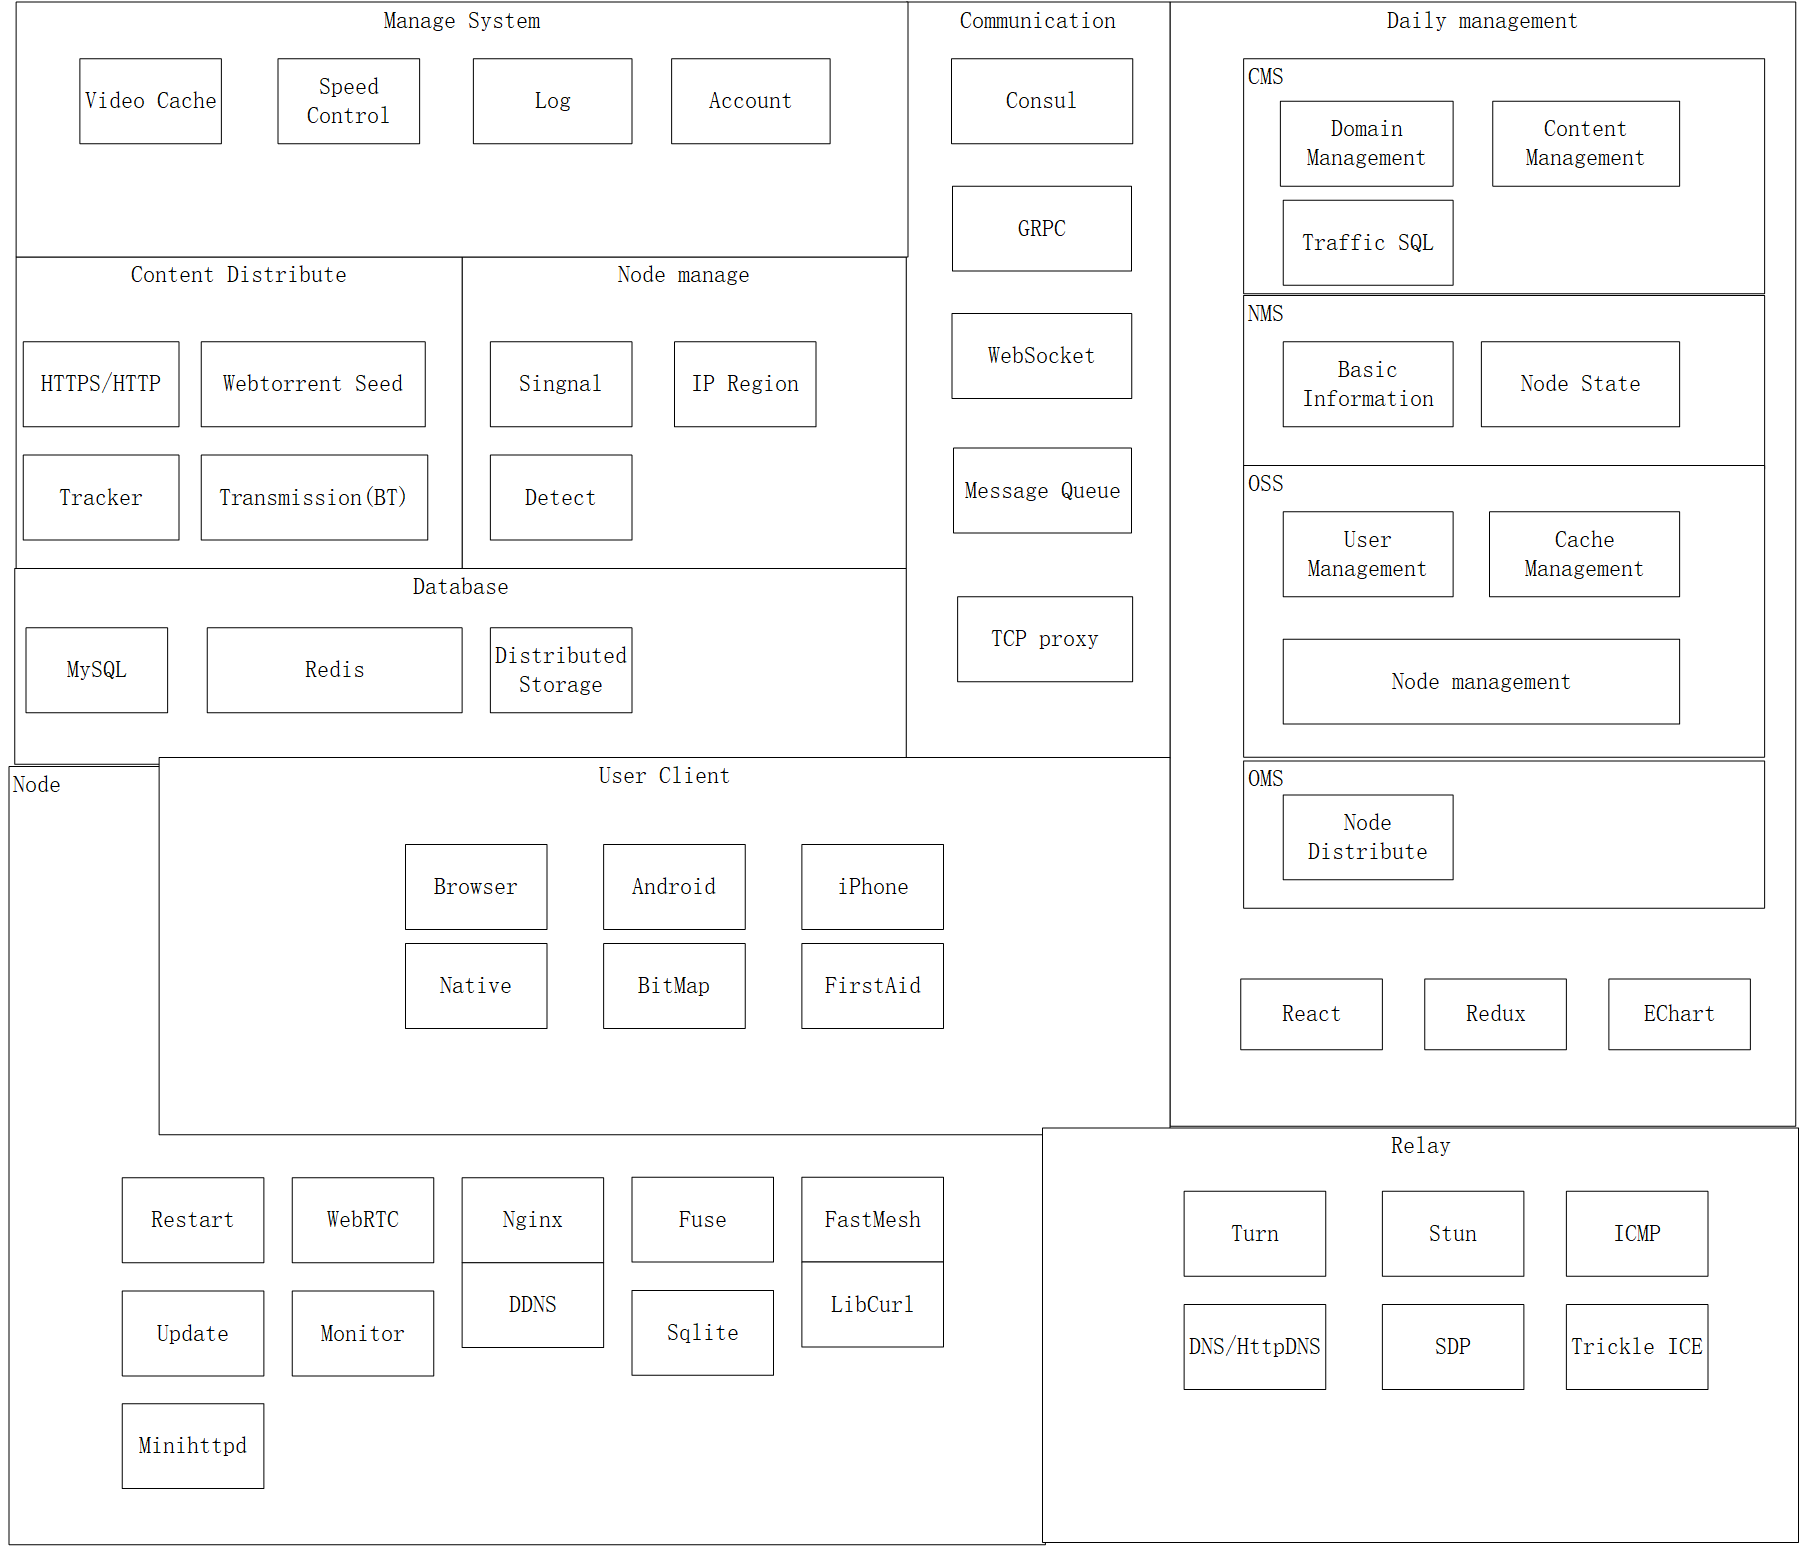
\includegraphics[width=\textwidth]{fig_6.png}
    \caption{Architecture of the Fog VDN}
	  \vskip 1.0cm
 \label{fig_6}
\end{figure}



Fog VDN is very simple(Figure \ref{fig_26}). The fog composed of the fog device
(such as Wi-Fi routers,Network Attached Storage,Smart home center,etc.) collect the
resources (bandwidth,storage,computing) combining cloud server to serve application X
(Fog as a Service FaaS,Figure \ref{fig_27}). But Fog VDN is also complex (Figure \ref{fig_6}),
composed by many systems. Whether simple or complex, Fog VDN has three subsystems,
Node System, Operations Management System and Network Protocols.

\begin{figure}[htbp]
\centering
	  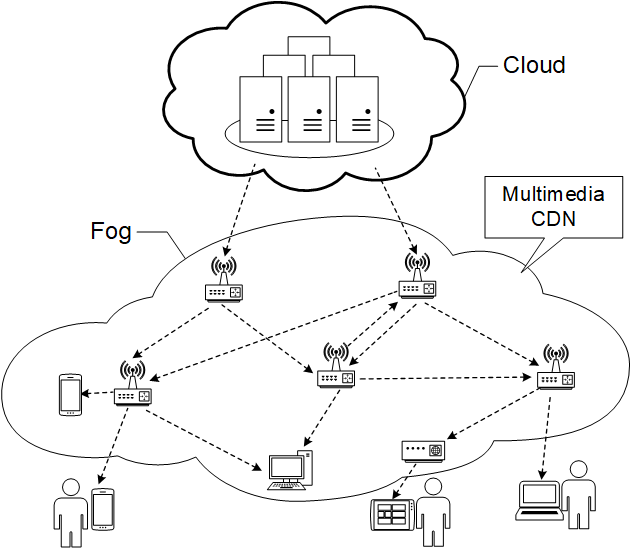
\includegraphics[width=0.8\textwidth]{fig_26.png}
    \caption{Simple architecture of the Fog VDN}
 \label{fig_26}
\end{figure}

\section{Node System}
 \label{Node System}
\begin{figure}[htbp]
\centering
	  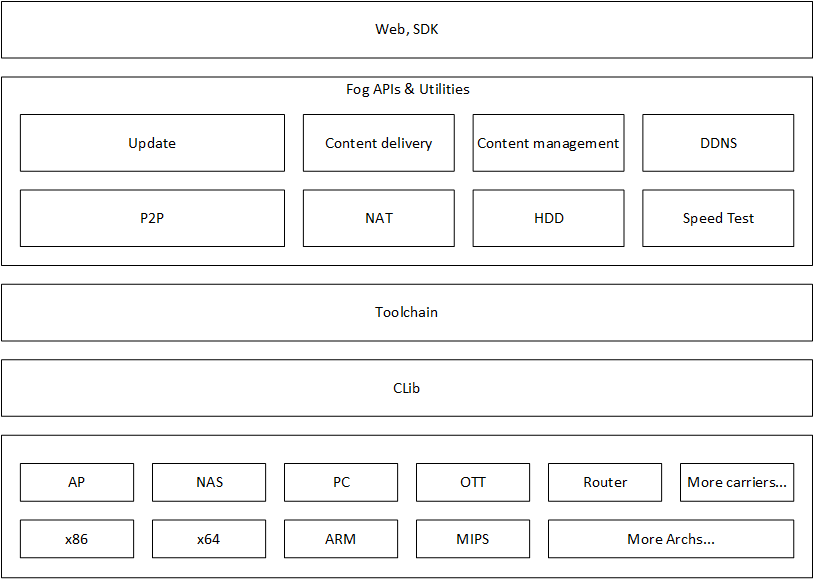
\includegraphics[width=\textwidth]{fig_25.png}
    \caption{ Architecture of the Fog nodes}
 \label{fig_25}
\end{figure}

  \subsection{Fog devices}
    \label{Fog devices}
  There are many different types about fog nodes, "Personal Computer"(PC), "Network Attached Storage"(NAS),
WirelessAccessPoint,Router,Mobile,Base Station all included. In this thesis, we only talk about the fog nodes
which can run the Fog VDN well, which generally have a large storage(>16GB), ROM(>32MB) and RAM(>512MB).
  For hardware devices, there are too many different platforms and configurations to easily unified.
Different from Xunlei and Youku product same hardware, also not same as Huawei use a heavy JVM platform,
 We use the C programing in order to minimize the size of program, so that it can run well in the fog
nodes and we can code once, compile everywhere.
 \subsection{Basic module}
    \label{Basic module}
  \begin{itemize}
    \item Node\_update  : update the program in node.
    \item Node\_restart : restart if the process broken down.
    \item Node\_monitor : monitor the process.
    \item Node\_report  : report the node basic information every 5 minutes.
    \item Node\_p2p     : connect to the other fog node.
    \item Node\_log     : record the node run time information.
    \item Node\_file    : manage the data in the nodes.
  \end{itemize}

  Fig \ref{fig_36} shows the relationship between these basic module.
 \subsection{General fog node}
 One of the most famous design philosophy of peer-to-peer system is sharing. As an application of P2P,
we also inherit the spirit of sharing. A special fog node  means the nodes which we refer to in section
\ref{Fog devices} . A general fog node include not only special fog node, but also the client. Figure
\ref{fig_34} is a fog player client, the red block is downloaded from the cloud, the blue, yellow and green
block is downloaded from special fog node. The purple block is downloaded from the client who is watching
this video. This is general fog node, same as conventional P2P node.
 Fig \ref{fig_25} shows the general fog node architecture.

\begin{figure}[htbp]
\centering
	  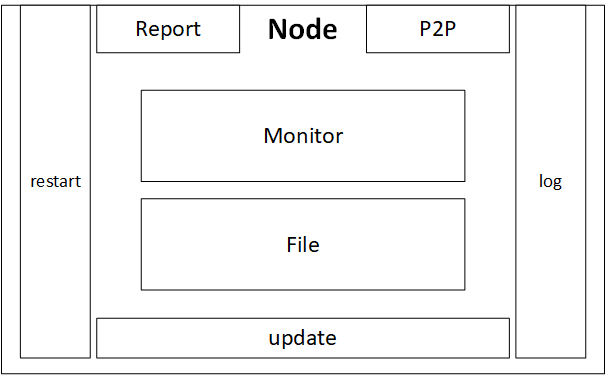
\includegraphics[width=0.8\textwidth]{fig_36.png}
    \caption{ Architecture of the Fog nodes System.}
 \label{fig_36}
\end{figure}

\section{Console}
\subsection{Operations Management System}
 \label{Operations Management System}
 Node system \ref{Basic module} have a basic module called Node\_report. The "Operations Management System"
(OMS) shows the statistics of these information (Figure \ref{fig_29}).
\begin{itemize}
	\item Amount                 : The number of fog nodes (\ref{Fog devices}).
	\item Amount\_online         : The number of fog nodes online.
  \item Bandwidth\_total       : The total upload/download bandwidth of fog nodes.
  \item Bandwidth\_total\_wan  : The total upload/download ability   of fog nodes.
  \item Bandwidth\_avg         : The average upload/download bandwidth of fog nodes.
  \item Bandwidth\_avg\_wan    : The average upload/download ability   of fog nodes.
  \item Storage\_total         : The total storage of fog nodes.
  \item Storage\_total\_able   : The available storage of fog nodes.
  \item NAT\_type              : The "Network Address Translation"(NAT) type.
  \item Platform               : The fog node's platform.
  \item HTTP                   : The node can support http connect.
  \item Version                : The node system version.
  \item Province               : The node province distribution.
  \item ISP                    : The node "Internet Service Provider"(ISP).
  \item Traffic                : The node traffic every 5 minutes.
\end{itemize}
  Figure \ref{fig_37} shows the relationship of these information.

\begin{figure}[htbp]
\centering
	  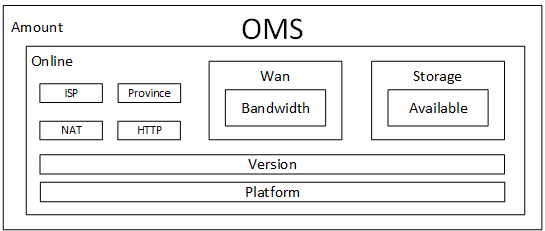
\includegraphics[width=0.8\textwidth]{fig_37.png}
    \caption{ Architecture of the OMS.}
 \label{fig_37}
\end{figure}

\subsection{Operation Supporting System}
The "Operation Supporting System" (OSS) is designed for administrator operating the fog nodes
(Figure \ref{fig_30}, Figure \ref{fig_32}).
\begin{itemize}
	\item Node\_list         :Similar to OSS (\ref{Operations Management System}), specific to each node.
  \item Update             : Update program by province, city, ISP, platform and current version.
  \item Update\_state      : Node update state.
  \item Version            : Node version distribution.
  \item Traffic            : Used traffic.
  \item Bandwidth          :Realtime bandwidth.
  \item Cache\_info        : Show the video uploaded information, include file\_name, host\_name, request\_url, distribute\_scheme, distribute\_status, upload\_time, finish\_time.
  \item Cache\_management  : Include upload, delete, change\_popularity, set\_url.
\end{itemize}


\subsection{Node Management System}
The "Node Management System" (NMS) is designed for user managing their fog device(Figure \ref{fig_38}).
\begin{itemize}
	\item User\_info     : User information include user name, email and phone.
  \item User\_coin     : User rewards for share their fog device.
  \item Node\_list     : User fog nodes list include "Media Access Control"(MAC), "Serial Number"(SN), NAT\_type, platform, version, province, ISP.
  \item Node\_state    : Node online or not.
  \item Node\_config   : Node configure.
\end{itemize}

\section{Application}
 In order to give an example that how to use the fog resource, we opensource a fog player.
Fig \ref{fig_7} show the architecture of this fog player.
\begin{figure}[htbp]
\centering
	  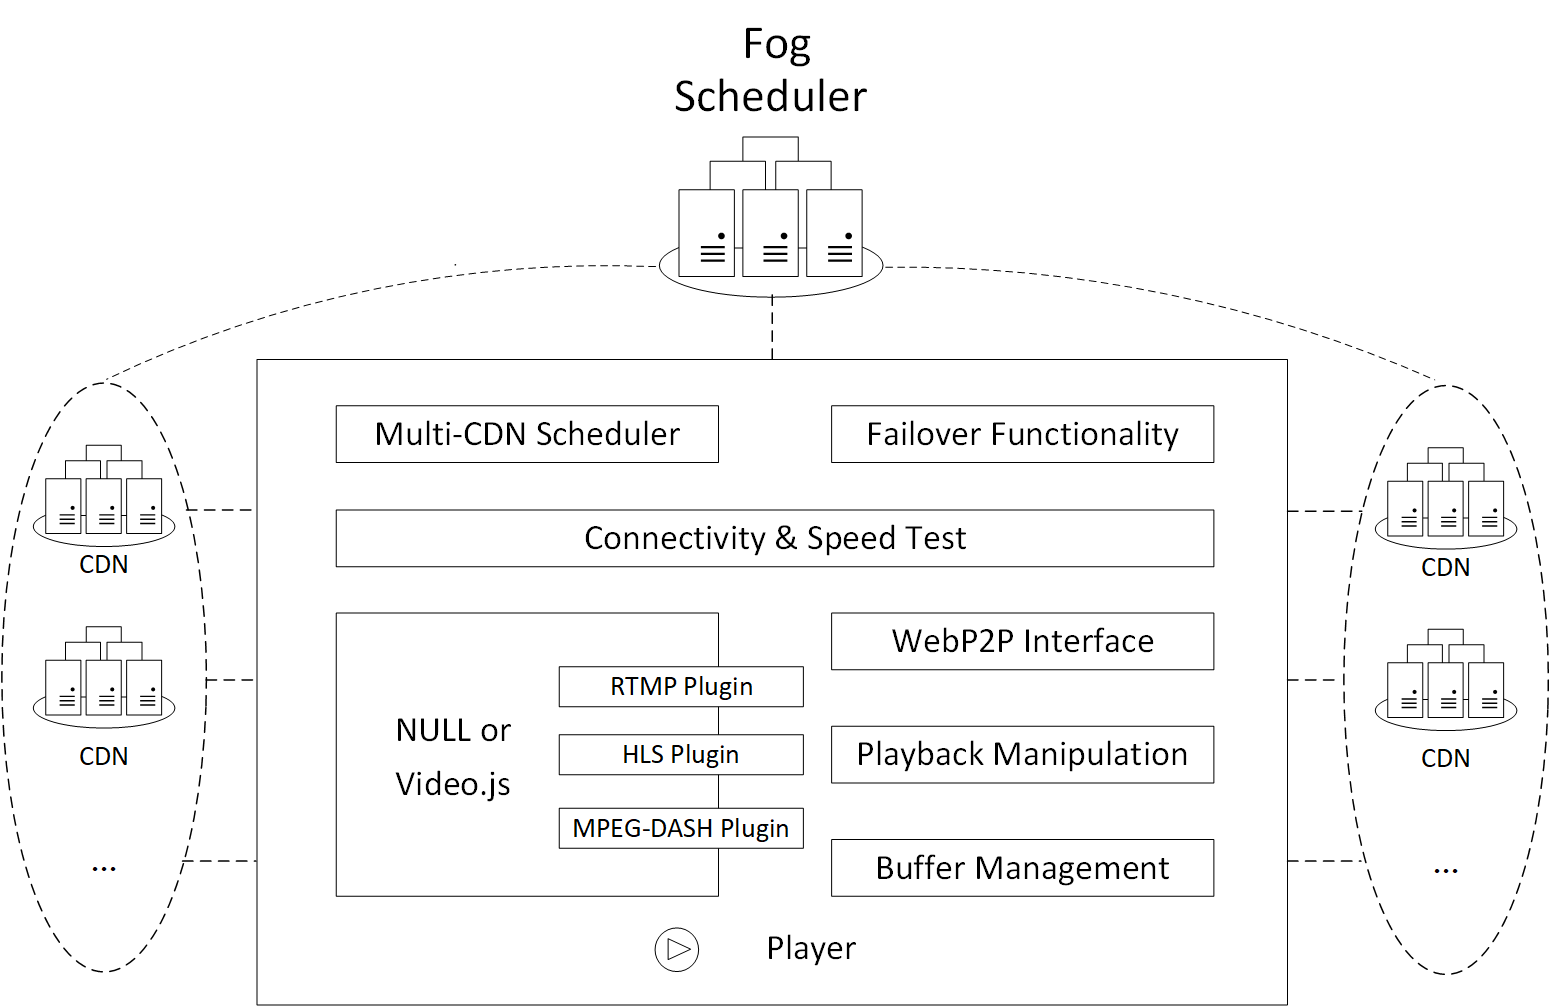
\includegraphics[width=\textwidth]{fig_7.png}
    \caption{Architecture of the Fog Player}
	  \vskip 1.0cm
 \label{fig_7}
\end{figure}

\section{Protocols}
In section \ref{Node System} we show a figure \ref{fig_25} of the architecture of fog nodes.
But if you were careful enough, you would find it is more protocol than system. We try to not only
conding a fog video distribution system but also summarizing a "Fog Video Distribution Network"(Fog VDN)
which focuse on protocol.Figure \ref{fig_8} and Figure \ref{fig_17} shows the fog node engine and Fog VDN stack.

Though we realized a fog video distribution sysem, and try to summarize some standards of connecting
the fog nodes as a network. But it is far away from a protocol, we still have a long way to go.


\begin{figure}[htbp]
\centering
	  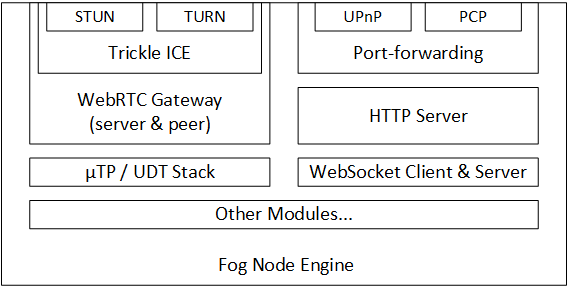
\includegraphics[width=0.8\textwidth]{fig_8.png}
    \caption{Architecture of the Fog Node Engine}
 \label{fig_8}
\end{figure}

\begin{figure}[htbp]
\centering
	  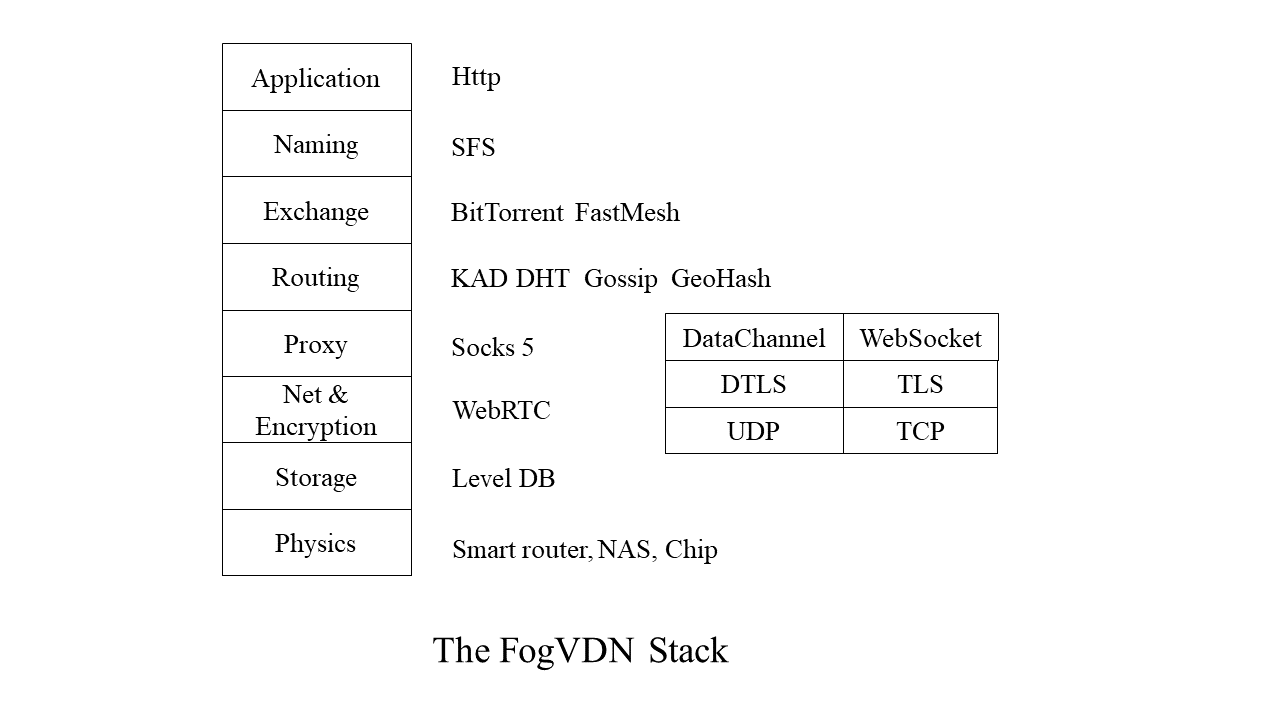
\includegraphics[width=\textwidth]{fig_17.png}
    \caption{Fog VDN Stack}
 \label{fig_17}
\end{figure}
